\documentclass[11pt,a4paper]{article}

\usepackage[T1]{fontenc}
\usepackage[utf8]{inputenc}
\usepackage[english]{babel}
\usepackage{lmodern}
%\usepackage{circuitikz}
\usepackage{color}
\usepackage{wrapfig}
\usepackage{placeins}
\usepackage{subfigure}
\usepackage{tabu}
\usepackage{fullpage}
\usepackage[squaren]{SIunits}
\usepackage{graphicx}
%\usepackage[pdftex]{graphicx}
\usepackage{epstopdf}
\usepackage{epsfig}
\usepackage{hyperref}
\usepackage{tikz}
\usepackage{tikz-qtree}
\usepackage{eurosym}
%\usepackage{chemist}
\usepackage{amsmath}
\usepackage{amssymb}
\usepackage{mathrsfs}
\usepackage{dsfont}% use $\mathds{1}$
\newcommand{\C}{\mathbb{C}}
\newcommand{\N}{\mathbb{N}}
\newcommand{\Z}{\mathbb{Z}}
\newcommand{\R}{\mathbb{R}}
\newcommand{\red}{\textcolor{red}}
\newcommand{\dis}{\displaystyle}
\newcommand{\dr}{\partial}
\newcommand{\txt}{\text}
\newcommand{\td}{\todo[inline]}
\newcommand{\ttt}{\texttt}
\newcommand{\itt}{\textit}

\usepackage{algorithm}
\usepackage{todonotes}
\usepackage[noend]{algpseudocode}

%\newtheorem{theoreme}			     {Théorème}	[chapter]
%\newtheorem{proposition}[theoreme]	 {Proposition}	
%\newtheorem{corollaire}	  [theoreme]	 {Corollaire}	
%\newtheorem{lemme}	      [theoreme]  {Lemme}		
%\newtheorem{definition}	         {Définition}[chapter]
%\theoremstyle{definition}
%\newtheorem{exemple}			     {Exemple}	[chapter]
%\newtheorem{contreexemple}[exemple]{Contre-exemple}
%\newtheorem{probleme}	             {Probl\`eme}[chapter]

\usepackage{listings}
\usepackage{textcomp}
\definecolor{listinggray}{gray}{0.9}
\definecolor{lbcolor}{rgb}{0.9,0.9,0.9}
\lstset{
	backgroundcolor=\color{lbcolor},
	tabsize=4,
	rulecolor=,
	language=matlab,
        basicstyle=\scriptsize,
        upquote=true,
        aboveskip={1.5\baselineskip},
        columns=fixed,
        showstringspaces=false,
        extendedchars=true,
        breaklines=true,
        prebreak = \raisebox{0ex}[0ex][0ex]{\ensuremath{\hookleftarrow}},
        frame=single,
        showtabs=false,
        showspaces=false,
        showstringspaces=false,
        identifierstyle=\ttfamily,
        keywordstyle=\color[rgb]{0,0,1},
        commentstyle=\color[rgb]{0.133,0.545,0.133},
        stringstyle=\color[rgb]{0.627,0.126,0.941},
}

\DeclareMathOperator{\e}{e}

\title{Titre}
\author{David Weicker}
\date{\today}

\begin{document}
\tabulinesep=1.2mm
\begin{center}
\hrule
\begin{tabular}{c}
\\[0.005cm]
\Large{SF2520 - Laboratory 7}\\[0.3cm] %THIS IS THE TITLE
\textsc{Goyens} Florentin  \& \textsc{Weicker} David \\[0.2cm]
$\text{26}^{\text{th}}$ November 2015\\[0.2cm] %THIS IS THE DATE
\end{tabular}
\hrule
\end{center}

\section*{Introduction}

This report answers the question given in the seventh laboratory for the course SF2520 - "Applied Numerical Methods". This laboratory is in the numerical algebra part. The first question concerns a stable QR-factorization for ill-posed systems and the second is about solving the least squares problem using a QR-factorization.

\section{Stable QR-factorization}

blabla
 
\section{Least Squares with QR-factorization}

This section tries to fit the data given with the least squares method. The function used to fit the data is :

$$y(t) = c_1 + c_2e^{\alpha t}+\sum_{k=1}^n (a_k cos(\frac{2\pi kt}{12}) + b_k sin(\frac{2\pi kt}{12}))$$

The problem consists thus of finding $c_1$, $c_2$, $a_k$ and $b_k$ that minimize $||Ax-b||_2$ where:

$$A = \left(\begin{array}{cccccccc}
1 & e^{\alpha t_1} & cos(\frac{2\pi k_1t_1}{12}) & \dots & cos(\frac{2\pi k_nt_1}{12}) & sin(\frac{2\pi k_1t_1}{12}) & \dots & sin(\frac{2\pi k_nt_1}{12}) \\ 
\vdots & \vdots & \vdots & \vdots & \vdots & \vdots & \vdots & \vdots \\ 
1 & e^{\alpha t_m} & cos(\frac{2\pi k_1t_m}{12})& \dots & cos(\frac{2\pi k_nt_m}{12}) & sin(\frac{2\pi k_1t_m}{12}) & \dots & sin(\frac{2\pi k_nt_m}{12})
\end{array} \right)$$

$$x=(c_1 \: c_2 \: a_1 \: \dots \: a_n \: b_1 \: \dots b_n)^T$$

And $b \in \mathbb{R}^{m\times 1}$ is the vector containing the data at times $t_i$ with $i=1...m$.

This problem can be solved using the least squares method. To do this, we are going to use the QR-factorization, i.e. the fact that:
$$A=QR$$

With $Q$ an orthogonal matrix and $R$ upper triangular. Indeed, to minimize the norm of the residual, we know that we have to solve the normal equations :
$$A^TAx=A^Tb$$

But using QR-factorization allows us to say (the proof that be found in the course notes) : 
$$Rx=Q^Tb$$

The Matlab code used to solve the problem can be found at the end of this report.

For $n=1$, here are the values obtained for the parameters :

\begin{center}
\begin{tabular}{|c|c|}
\hline 
$c_1$ & 2.5581 \\ 
\hline 
$c_2$ & 334.9964 \\ 
\hline 
$a_1$ & -1.7186 \\ 
\hline 
$b_1$ & 2.3581 \\ 
\hline 
\end{tabular} 
\end{center}

And the computed norm of the residual is :
$$||res(n=1)||_2=15.2036$$

For $n=2$, the parameters are the following : 

\begin{center}
\begin{tabular}{|c|c|}
\hline 
$c_1$ & 2.7340 \\ 
\hline 
$c_2$ & 334.8298 \\ 
\hline 
$a_1$ & -1.7185 \\ 
\hline 
$a_2$ & 0.8382 \\
\hline
$b_1$ & 2.3579 \\ 
\hline 
$b_2$ & -0.0345\\
\hline
\end{tabular} 
\end{center}

And the norm of the residual is :
$$||res(n=2)||_2=11.3936$$

And finally, for $n=3$, these are the parameters : 

\begin{center}
\begin{tabular}{|c|c|}
\hline 
$c_1$ & 2.7665 \\ 
\hline 
$c_2$ & 334.7990 \\ 
\hline 
$a_1$ & -1.7185 \\ 
\hline 
$a_2$ & 0.8382 \\
\hline
$a_3$ & 0.1094\\
\hline
$b_1$ & 2.3579 \\ 
\hline 
$b_2$ & -0.0345\\
\hline
$b_3$ & -0.0568\\
\hline
\end{tabular} 
\end{center}

And the norm of the residual is :
$$||res(n=3)||_2=11.2972$$

It is important to note that the norm of the residual decreases as we increase $n$. That is to be expected since when we increase $n$ by one, we allow two new degrees of freedom. Thus, it is not possible to obtain a "worse" residual with a higher $n$. In the worst case scenario, the two new basis functions do not increase the quality of the fitting and then the corresponding coefficients would be zero. The residuals would then be equal.

Figure \ref{lsp} shows the fitting for $n=3$. We can see that it is relatively good. The $'x'$ are the data points and the red curve is the fitting.

\begin{figure}
\begin{center}
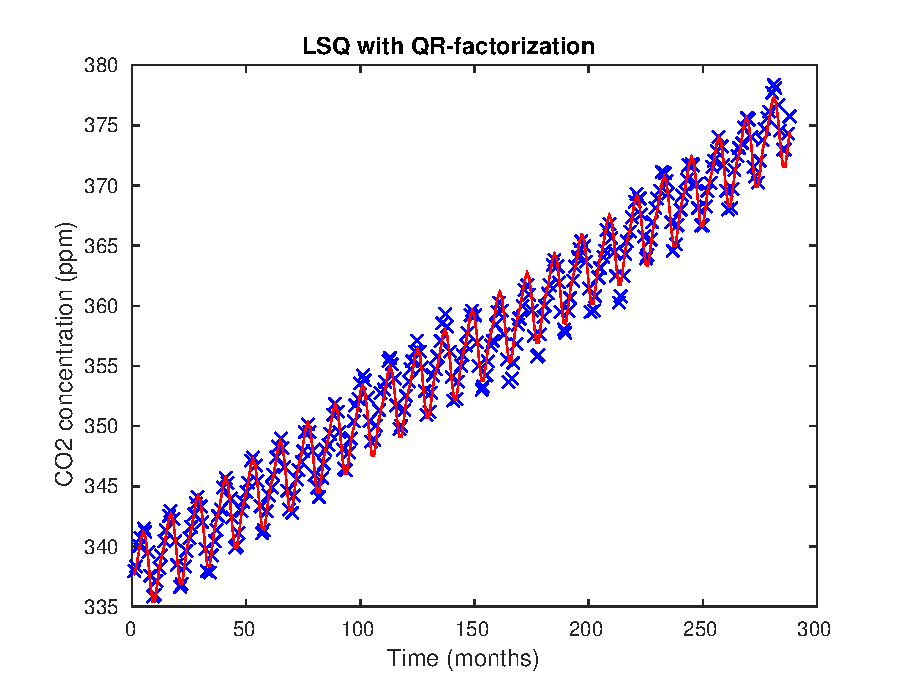
\includegraphics[scale=0.5]{lsp.eps}
\caption{Fitting of the data for $n=3$}
\label{lsp}
\end{center}
\end{figure}


\newpage
\section{Code Listing}

\lstinputlisting{qrFact.m}
\newpage
\lstinputlisting{lsp.m}

\end{document}